\section[Projeto de Detectores Luminosos]{Projeto de Detectores Luminosos}
\label{sec_circ_comp}

Um circuito integrado foi desenvolvido para a comunicação de dados via luz, utilizando-se dos circuitos apresentados na \autoref{section:APS} e \autoref{section:TIA} deste documento. O projeto \'e representado em alto n\'ivel na \autoref{fig_circcompleto}. Todos os sinais aqui apresentados na figura, e tamb\'em em todas figuras \`a seguir, seguem o a padr\~ao descrito na \autoref{section:padrao_sinais} deste trabalho.

\begin{figure}[htb]
	\caption{\label{fig_circcompleto}Circuito projetado}
	\begin{center}
	    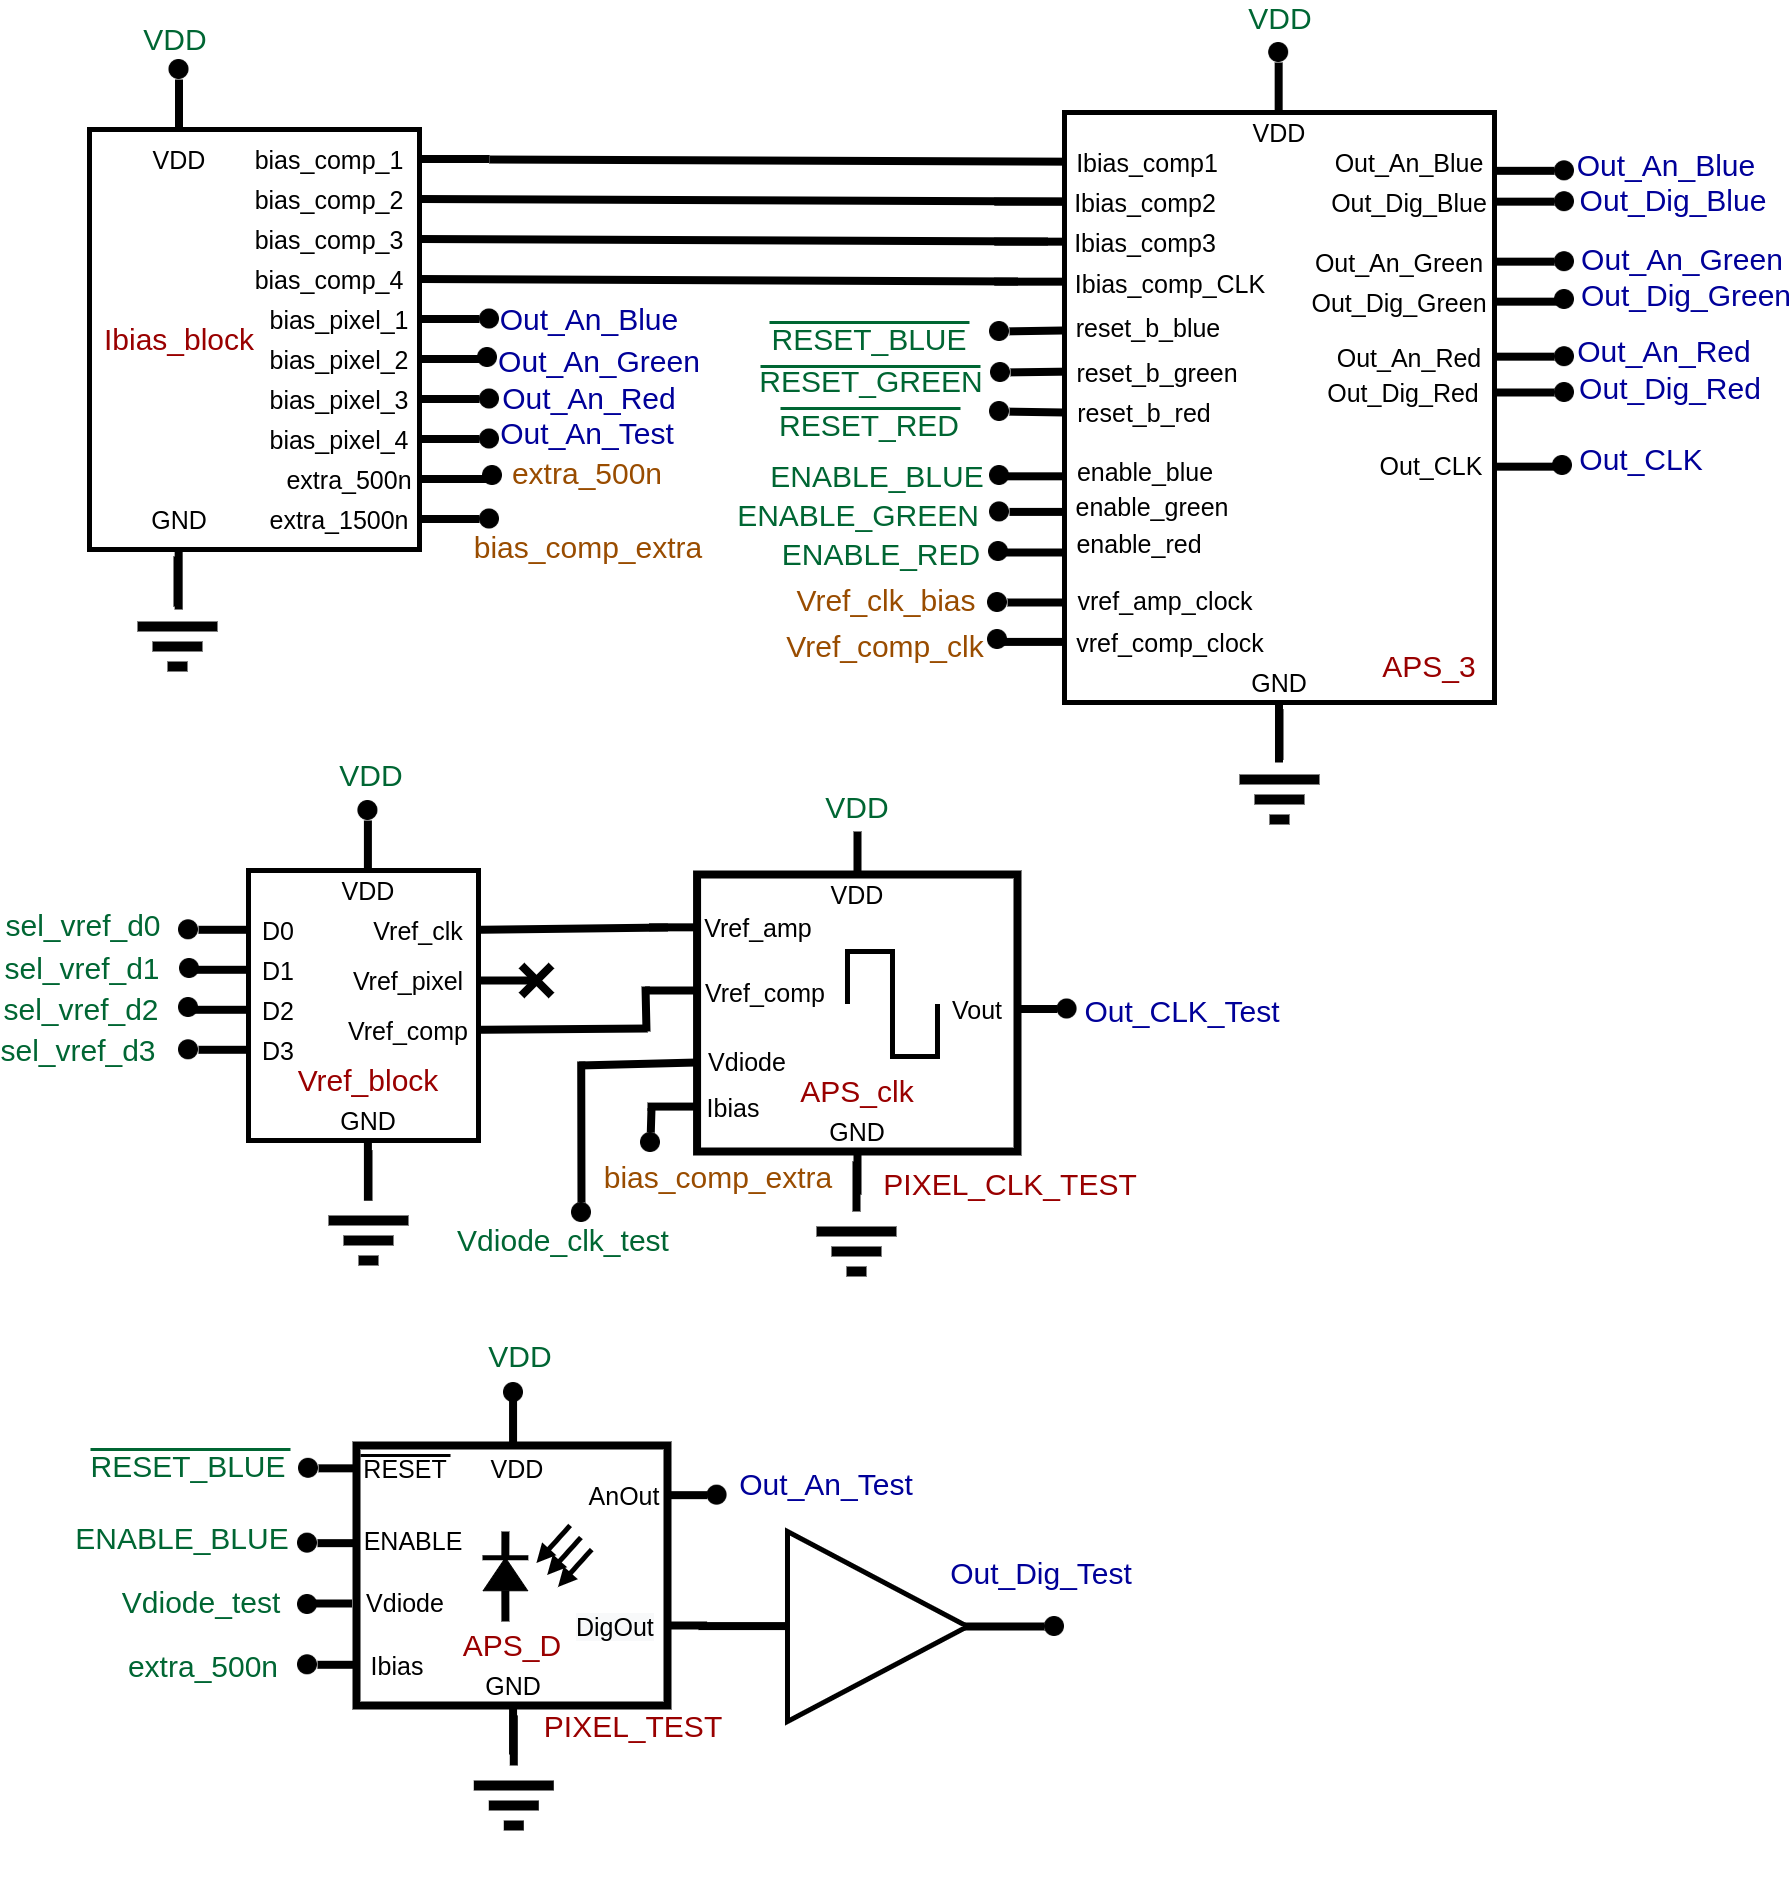
\includegraphics[width=\textwidth]{Circuitos/Complete_Circuit.png}
	\end{center}
	\legend{Fonte: Produzido pelo autor}
\end{figure}

O circuito tem a finalidade de processar a informa{\c c}\~ao advinda de tr\^es \emph{APS}'s, constru\'idos de maneira id\^entica em n\'ivel de layout, com a finalidade de abstrair informa{\c c}\~oes de cores advindas de uma fonte luminosa, dos quais podem ser Azul, Verde ou Vermelha. Para que as cores fossem devidamente separadas entre cada \emph{APS}, filtros luminosos externos, por meio de uma pel\'icula colorida, s\~ao adicionados sob cada \emph{APS} respons\'avel por processar uma cor equivalente \`a de sua pel\'icula.

Um sinal luminoso de cor branca tamb\'em \'e utilizado no sistema de forma a ser a refer\^encia de rel\'ogio de todos \emph{APS's} descritos. Esse sinal \'e processado utilizando-se um $TIA$, do qual \'e gerado um sinal el\'etrico equivalente \'a informa{\c c}\~ao luminosa.

A tecnologia de fabrica{\c c}\~ao utilizada para o desenvolvimento de todos blocos foi a \emph{CMOS 180nm da TSMC}. O software utilizado para o projeto do dispositivo foi o \emph{Virtuoso}, desenvolvido pela \emph{Cadence}.

O circuito representado na \autoref{fig_circcompleto} \'e composto por 2 blocos principais, que permitem o processamento advindos da fonte luminosa, al\'em de um circuito \emph{APS} e um \emph{TIA} extra. A descri{\c c}\~ao dos bloco s\~ao:

\begin{itemize}
    \item \emph{ibias\_block}: Tem a fun{\c c}\~ao de gerar fontes de corrente utilizadas em alguns blocos do circuito.
    
    \item \emph{APS\_3}: Implementa os tr\^es circuitos \emph{APS} descritos, al\'em do circuito \emph{TIA}. A sa\'ida de cada bloco passa por um comparador de forma a digitalizar o dado, como ser\'a melhor explicitado na \autoref{sec_apsdigitalized}.
    
    \item \emph{Vref\_block} e \emph{PIXEL\_CLK\_TEST}: Estes blocos realizam a implementa{\c c}\~ao de um TIA, por\'em com a adi{\c c}\~ao de um pino extra que possibilita a simula{\c c}\~ao de uma corrente fotogerada sem necessitar de uma fonte luminosa. Estes blocos ser\~ao melhor explicados na \autoref{BlocoTestes}. 
    
    \item \emph{PIXEL\_TEST}: Este bloco realiza a implementa{\c c}\~ao de um APS, por\'em com a adi{\c c}\~ao de um pino extra que possibilita a simula{\c c}\~ao de uma corrente fotogerada sem necessitar de uma fonte luminosa. Este bloco será melhor explicado na \autoref{BlocoTestes}.
    
\end{itemize}

A \autoref{tab_circcomp} mostra a rela{\c c}\~ao de sinais de entrada e sa\'ida presentes no circuito, para o processamento dos p\'ixels de cor. A \autoref{tab_circcomp2} mostra a rela{\c c}\~ao de sinais de entrada e sa\'ida presentes no circuito para o processamento dos blocos de teste.

\begin{table}[htb]
\label{tab_circcomp}
\centering
\caption{Descri{\c c}\~ao dos sinais de entrada e sa\'ida do circuito projetado para as cores azul, verde e vermelha}%
  \begin{tabular}{ccll}
  \toprule
   Sinal & Tipo & Descri{\c c}\~ao & Observa{\c c}\~ao \\
  \midrule \midrule
   RESET\_BLUE & Entrada & \begin{tabular}[l]{@{}l@{}}Sinal de tensão de \emph{RESET}\\ no APS para cor azul\end{tabular}   & Ativo em n\'ivel baixo \\
  \midrule
   RESET\_GREEN & Entrada & \begin{tabular}[l]{@{}l@{}}Sinal de tensão de \emph{RESET}\\ no APS  para cor verde\end{tabular}   & Ativo em n\'ivel baixo \\
  \midrule
   RESET\_RED & Entrada & \begin{tabular}[l]{@{}l@{}}Sinal de tensão de \emph{RESET}\\ no APS  para cor vermelha\end{tabular}   & Ativo em n\'ivel baixo \\
  \midrule
   ENABLE\_BLUE & Entrada & \begin{tabular}[l]{@{}l@{}}Sinal de tensão de \emph{ENABLE}\\ no APS para cor azul\end{tabular}   & Ativo em n\'ivel alto \\
  \midrule
   ENABLE\_GREEN & Entrada & \begin{tabular}[l]{@{}l@{}}Sinal de tensão de \emph{ENABLE}\\ no APS para cor verde\end{tabular}   & Ativo em n\'ivel alto \\
  \midrule
   ENABLE\_RED & Entrada & \begin{tabular}[l]{@{}l@{}}Sinal de tensão de \emph{ENABLE}\\ no APS para cor vermelha\end{tabular}   & Ativo em n\'ivel alto \\
  \midrule
   Out\_An\_Blue & Sa\'ida & \begin{tabular}[l]{@{}l@{}}Sinal de tensão anal\'ogica\\ para cor azul\end{tabular} \\
  \midrule
   Out\_Dig\_Blue & Sa\'ida & \begin{tabular}[l]{@{}l@{}}Sinal de tensão digital\\ para cor azul\end{tabular} \\
  \midrule
   Out\_An\_Green & Sa\'ida & \begin{tabular}[l]{@{}l@{}}Sinal de tensão anal\'ogica\\ para cor verde\end{tabular} \\
  \midrule
   Out\_Dig\_Green & Sa\'ida & \begin{tabular}[l]{@{}l@{}}Sinal de tensão digital\\ para cor verde\end{tabular} \\
  \midrule
   Out\_An\_Red & Sa\'ida & \begin{tabular}[l]{@{}l@{}}Sinal de tensão anal\'ogica\\ para cor vermelha\end{tabular} \\
  \midrule
   Out\_Dig\_Red & Sa\'ida & \begin{tabular}[l]{@{}l@{}}Sinal de tensão digital\\ para cor vermelha\end{tabular} \\
   \midrule
   Out\_CLK & Sa\'ida & \begin{tabular}[l]{@{}l@{}}Sinal de tensão de rel\'ogio\\ gerado pelo TIA\end{tabular}\\
  \bottomrule
\end{tabular}%

\legend{Fonte: Produzido pelo autor.}
\end{table}

\begin{table}[htb]
\IBGEtab{%
  \caption{Descri{\c c}\~ao dos sinais de entrada e sa\'ida do circuito projetado para os blocos de teste}%
  \label{tab_circcomp2}
}{%
  \begin{tabular}{ccl}
  \toprule
   Sinal & Tipo & Descri{\c c}\~ao \\
   \midrule \midrule
   Vdiode\_test & Entrada & Corrente que simula um potencial no fotodiodo do APS de teste\\
   \midrule
   Vdiode\_clk\_test & Entrada & Corrente que simula um potencial no fotodiodo no TIA de teste\\
   \midrule
   Out\_An\_Test & Sa\'ida & Sinal de tensão anal\'ogico para o APS de teste \\
   \midrule
   Out\_Dig\_Test & Sa\'ida & Sinal de tensão digital para o APS de teste \\
  \midrule
   Out\_CLK\_test & Sa\'ida & Sinal de tensão de rel\'ogio gerado pelo TIA de teste\\
  \bottomrule
\end{tabular}%
}{%
  \fonte{Produzido pelo autor.}
}
\end{table}